\section{Operationally-defined preorders}

In this section, we consider our first approach to defining an admissible and compositional basic operational
preorder $\Basicleq$ on $\Trees(\mathbb{N})$. We call this method \emph{operational}. Its characteristic is that the preorder
 $\Basicleq$ is directly defined using a mathematical model of the way that an effect tree in $\Trees(\mathbb{\Nat})$ will be executed.

This approach is illustrated for several examples of effects in~\cite{gom}. 
The main goal of the section is to demonstrate the approach using a different example, the signature
$\Sigma_\prnd = \{\prEff,\orEff\}$ from Example~\ref{example:prnd}, which is of interest because of the 
interplay between probabilistic and nondeterministic effects. However, we first
briefly review the simpler cases, $\Sigma_\pr = \{\prEff\}$ and $\Sigma_\nd = \{\orEff\}$, of purely probabilistic and 
purely nondeterministic computation. Since these cases are relatively simple, and are already covered in~\cite{gom},
our treatment will be brief.

First, we  consider the case $\Sigma_\pr = \{\prEff\}$. Every internal node in a  tree $t \in \Trees(\mathbb{N})$  is a binary branching node labelled with $\prEff$ representing a probabilistic choice with each branch having probability $\frac{1}{2}$. The tree can thus be interpreted as a (countable state) Markov-chain, that determines a discrete subprobability distribution over the set $\mathbb{N}$.
(It is a subprobability distribution because there can be a positive probability of nontermination, both silent and noisy.) We write
$\mathbf{P}_t (n)$ for the probability assigned to the return value $n$ by the tree $t$.
The basic operational preorder is defined by:
\[
t \Basicleq_\pr t' ~ \Leftrightarrow ~ \forall n ~ ~ \mathbf{P}_t (n) \leq \mathbf{P}_{t'}(n) \enspace .
\]
\begin{aproposition}
The relation $\Basicleq_\pr$ is an admissible compositional preorder. 
\end{aproposition}
\noindent
It is also possible to define $\Basicleq_\pr$ cas $\Basicleq_{\mathcal{O}_\pr}$ for the a family of Scott-open subsets of $\Trees(\mathbb{N})$, \emph{viz}:
\[
\mathcal{O}_\pr ~ = ~ \{\,  \{t \mid \mathbf{P}_t (n) > q\} \mid n \in \mathbb{N}, \,q \in \mathbb{Q}\, \}  \enspace .
\]

Next, we consider the case $\Sigma_\nd = \{\orEff\}\,$. In this case,  every internal node in a tree is a binary nondeterministic choice.
Typically nondeterminism models a choice that will be made by some external agent, called the \emph{scheduler}, over whom we have no control. We can  model the scheduler as resolving the nondeterminism by specifying a scheduling 
function $s: \{l,r\}^* \to \{l,r\}$. The idea is that a word $w \in \{l,r\}^*$ represents a finite path of left/right choices from the root of a 
tree $t \in \Trees(\mathbb{N})$. If the computation reaches a nondeterministic choice at the node indexed by 
$w$ then it takes the left/right branch according to the value of $s(w)$. This way of representing choices has some redundancy
(in every tree other than the complete infinite binary tree, there will be words $w$ that do not index nodes in the tree; if $s(\varepsilon) = l$ then the value of $s$ on words beginning with $r$ is immaterial; etc.), but it is simple and convenient for future purposes. 
Given such a scheduling function $s$, we write $t@s$ for the result of the computation as scheduled by $s$. This is defined by:
\[
t@s ~ = ~ \begin{cases} 
 n & \text{if there exists $w \in \{l,r\}^*$ indexing an $n$ node in $t$} \\
    & ~~~\text{such that, for every $i < |w|$, $~w_{i+1} = s(w\!\restriction_i)\,$;} \\
  \bot & \text{otherwise.}
 \end{cases}
\]
Here we write $|w|$ for the length of a word, $w_i$ for the $i$-th symbol in a word, and $w \!\restriction_i$ for the prefix of $w$ that has length $i$.

The  \emph{angelic} interpretation of nondeterminism takes into account the possibility of a nondeterministic computation achieving a specified goal, given a cooperative scheduler.  The  \emph{demonic} interpretation, 
models the {necessity} that a goal will be achieved, however adversarial the scheduler. For effect trees in $\mathbb{N}$, goals are naturally specified as sets $G \subseteq \mathbb{N}$ of desired return values. One is then interested in the possibility or necessity 
that a scheduler produces a value in $G$. This leads to the definitions below, where the statement $t@s \in G$ implies in particular that $t@s \neq\bot$.
\begin{align*}
t \Basicleq_\ang t' ~ \Leftrightarrow ~ ~& \forall G \subseteq \mathbb{N}~~ (\exists s ~\; t@s \in G)~ \Rightarrow~ (\exists s ~ \; t'@s \in G) 
\\
t \Basicleq_\dem t' ~ \Leftrightarrow ~ ~& \forall G \subseteq \mathbb{N}~~ (\forall s ~ \; t@s \in G)~ \Rightarrow~ (\forall s ~ \; t'@s \in G) 
\end{align*}
\begin{aproposition}
The preorders $\Basicleq_\ang$  and $\Basicleq_\dem$ are admissible and compositional. 
\end{aproposition}


In the case of combined (demonic) non-determinism and probabilities we can define 
the preorder $\sqeq_b$ on trees over natural numbers in a simple and
effective way. We consider a tree as a Markov Decision Process 
and given an cost function from $\Nat \to \overline{\mathbb{R}_+}$
we find a strategy for the $\orEff$ nodes that minimizes the average
cost of the tree. 

A tree $t$ is under a tree $t'$ for this preorder when for any 
cost function, the minimal expected cost for $t$ is under the 
minimal expected cost for $t'$.

In order to formalise this intuition, while not diving into the details of 
all the specifications one can 
define $\mathcal{S}$ to be the space representing 
the set of strategies. Given a strategy $s \in \mathcal{S}$ and 
a tree $t \in \Tree_\Nat$, one can build $t*s$ the application of 
the strategy to the tree, that builds a new \emph{probability} tree, that 
is \emph{without} $\orEff$ nodes. Given a probability tree $t$, and a 
cost function $h$ from $\Nat$ to $\overline{\mathbb{R}_+}$, one can define the expected cost $\mathbb{E} (h(t))$.
It is now possible to write the following definition for the operational 
preorder:

\begin{equation*}
    t \sqeq_b t' \iff 
    \forall h : \Nat \to \overline{\mathbb{R}_+}, 
    \inf_{s \in \mathcal{S}} \mathbb{E}(h(t*s)) \leq 
    \inf_{s \in \mathcal{S}} \mathbb{E}(h(t'*s))
\end{equation*}

Admissibility is going to rely on the \emph{Scott-continuity} 
of the following function:

\begin{equation*}
    t \mapsto \left(h \mapsto \inf_{s \in \mathcal{S}} \mathbb{E} (h
(t*s))\right)
\end{equation*}

Compositionality on the other hand is going to rely on an elementary 
decomposition result of the above function.

\subsection{Formalisation of strategies} 

The goal of this subsection is to formalise strategies and 
to build a \emph{continuous} function from $\Tree_\Nat \times \mathcal{S}$
to $\Tree_\Nat$ (without $\orEff$ nodes) corresponding to the 
application of a strategy to a tree.
The first step to define strategies is to define the space 
$\{ L; R\}$ of directions that can be taken in the tree (left and right).
Using this set, one can define the set of paths as $\{ L; R \}^*$. A 
strategy can be seen as a function that takes a path as input (position 
in a tree) and outputs the direction to choose.

\begin{adefinition}[Strategies]
     The set of strategies is 
     defined by $\mathcal{S} = \{ L;R\}^* \to \{ L; R\}$.
     This set is compact for the topology induced by the 
     following distance on strategies:

     \begin{equation*}
         d(s_1,s_2) = \inf_{n \geq 1} \left\{ \frac{1}{n} ~|~ \forall p \in \{ L;R\}^*,
                                         |p| \leq n, s_1(p) = s_2(p) \right\}
     \end{equation*}
\end{adefinition}

\begin{proof}
    The function $d$ is clearly a distance and a converging sequence 
    of strategies can be extracted from any other one by the usual argument 
    (looking at the output on the empty sequence, and then extracting
    infinitly many elements from the sequence outputting the same thing etc.).
\end{proof}

Now that we have theses functions, we can define the space 
of strategies evaluations that are \emph{continuous}
functions from the cantor space to trees. 

This construction may seem unnatural, but it is the simplest 
way to get continuity of strategy application to a tree.

\begin{adefinition}[Application space]
    The space $\mathcal{C}(S,\Tree_\Nat)$ is a $\Sigma$-continuous 
    algebra where:

    \begin{equation*}
        \orEff (e_1,e_2) (s) = 
        \begin{cases}
            e_1 (s \circ L) & \text{when } s(\varepsilon) = L \\
            e_1 (s \circ R) & \text{when } s(\varepsilon) = R 
        \end{cases}
    \end{equation*}

    And where:
    \begin{equation*}
        \prEff (e_1,e_2) (s) = \prEff (e_1 (s \circ L), e_2 (s \circ R)) 
    \end{equation*}

    With $L$ and $R$ being considered interpreted as the function 
    from paths to paths that appends the corresponding letter in front of 
    the path.
\end{adefinition}

Now that we have this space of function, we can define the 
homomorphism that maps a tree to a function from strategies 
to trees, that is the curryfication of the function we want to build.

\begin{adefinition}[Strategy Application]
    We define the function $*$ from $\Tree_\Nat$ to $\mathcal{C}(\mathcal{S},\Tree_\Nat)$
    as the unique homomorphism such that:

    \begin{enumerate}
        \item $n* = s \mapsto n$
        \item $\bot* = s \mapsto \bot$
    \end{enumerate}
\end{adefinition}

Note that during this definition, we actually defined very precisely 
how strategies apply, and it is straightforward to check that 
application works as expected.

\begin{alemma}[Continuity]
    Given a tree $t$ and a strategy $s$ we can 
    build a tree $(t*) (s)$. The function 
    $\operatorname{app}(t,s) = (t*)(s)$ written sometimes
    $(t*s)$ 
    is continuous 
    from $\Tree_\Nat \times \mathcal{S}$ to $\Tree_\Nat$.
\end{alemma}

\begin{proof}
    It is clear that $(t*s)$ is continuous in each of it's 
    arguments. Using the fact that $\Tree_\Nat$ is a 
    continuous domain we can use a well know fact 
    \cite{battenfeld2009two} (Lemma A.1) that allows us to conclude.
    \qed
\end{proof}


\subsection{Formalisation of probabilities}

Now that we can get a tree without \texttt{or} nodes,
we can define the probability space we are using, mainly 
infinite paths on binary trees, corresponding to real numbers.

\begin{adefinition}[Probability Space]
    We define the probability space $\Omega$
    to be $\{0,1\}^\mathbb{N}$, the 
    $\sigma$-algebra to be the Borel sets 
    and use the uniform probability measure on them.
\end{adefinition}

Any tree can then be turned into a random variable in 
a very natural way. 

\begin{adefinition}[Turning a tree into a random variable]
    Given a tree $t$ with only \texttt{or} nodes we 
    build a measurable function $va(t)$ from $\Omega$ to $\Tree_\Nat$:

    \begin{equation*}
        va(t)(p) = \begin{cases}
            n  & \text{ if there is a node } n \text{ on the path } p \\
            \bot & \text{ otherwise } 
        \end{cases}
    \end{equation*}
\end{adefinition}

%\begin{proof}
    %The random variable for a given tree is a measurable function 
    %in an obvious way.
%\end{proof}

\subsection{Construction of the preorder}

We now have all the constructions needed to define the preorder

\begin{adefinition}[Preorder]
    The preorder is defined by

    \begin{equation*}
        t \sqeq_b t' \iff \forall h : \Nat \to \overline{\mathbb{R}_+}, 
        \inf_{ s \in \mathcal{S}} F (t,s,h) \leq \inf_{s \in \mathcal{S}} F (t',s,h)
    \end{equation*}

    Where the function $F$ is defined as 

    \begin{equation*}
        F(t,s,h) = \mathbb{E}(h \circ va(t * s))
    \end{equation*}
\end{adefinition}

To prove the admissibility, it suffices to prove that the function 
is Scott-continuous, and we made sure that this fact is easy to prove.

\begin{alemma}[Scott-continuity]
    Given a cost function $h$, the function 
    $(t,s) \mapsto F(t,s,h)$ is continuous from $\Tree_\Nat \times
    \mathcal{S}$ with the product topology to $\overline{\mathbb{R}_+}$ with the 
    Scott topology.

    Moreover, given $t$ and $s$, the function $h \mapsto F(t,s,h)$ is monotone.
\end{alemma}

\begin{proof}
    We write $RV(X)$ for the space of random variables 
    that have values on $X$, that is measurable 
    functions from $\Omega$ to $X$. Moreover when 
    $X$ is $\mathbb{N}_\bot$ or $\overline{\mathbb{R}_+}$
    we can use the Scott topology on $X$ and notice that in both cases 
    measurable functions are closed under directed suprema 
    allowing us to consider $RV(\mathbb{N}_\bot)$ and $RV(\overline{\mathbb{R}_+})$ as 
    domains.

    \begin{center}
        \begin{tikzcd}
            \Tree_\Nat \arrow[r, "va"] & 
            RV( \mathbb{N}_\bot ) \arrow[r, "h \circ"] &
            RV(\overline{\mathbb{R}_+}) \arrow[r, "\mathbb{E}(\square)"] & 
            \overline{\mathbb{R}_+}
        \end{tikzcd}
    \end{center}

    This function is Scott-continuous as a composition of 
    Scott-continuous functions. Indeed $va$ is clearly Scott-continuous 
    by definition, left composition with a function is also
    Scott-continuous, and the expectancy is a monotone operator 
    that preserves directed suprema via the monotone convergence theorem. 

    We can then say that $F(t,s,h)$ is continuous at a fixed $h$
    because it is the composition of $(t*s)$ with a Scott-continuous 
    function.

    \qed
\end{proof}

Now the last bit is showing that taking the infimum gives 
a continuous function in $(s,t)$ that is still monotone on $h$.
This follows from a general result using the compactness of the 
set of strategies and the continuity of the functions 
\cite{AndreaShalk} (Theorem 7.31).

\begin{alemma}[Taking the infimum]
    \label{lem:mixedscottcontinuous}
    Fixing $h$ and $s$, 
    the function $t \mapsto \inf_s \mathbb{E} (h \circ va(t*s))$
    is Scott-continuous.
\end{alemma}

\begin{proof}
    It is possible to use a result from Andrea Shalk's thesis 
    \cite{AndreaShalk} (Theorem 7.31)
    to directly prove the result. Note that 
    the compactness of $S$ is a crucial hypothesis. 

    It is also possible to build a direct proof of Scott-continuity:
    first of all monotonicity is simply obtained because an infimum 
    of monotone functions is monotone. Then, the only result left 
    to prove is that given an ascending chain of trees $(t_i)_{i \in \mathbb{N}}$
    we have the following equation:

    \begin{equation*}
        \sup_{i \in \mathbb{N}} \inf_{s \in \mathcal{S}} F(t_i,s,h) = 
    \inf_{s \in \mathcal{S}} F (\sqcup_i t_i, s, h)
    \end{equation*}
    
    Because $F$ is Scott-continuous in $t$, we can rewrite the right hand 
    side of the equality, and obtain the following inequality: 

    \begin{equation*}
        \sup_{i \in \mathbb{N}} \inf_{s \in \mathcal{S}} F(t_i,s,h) \leq 
        \inf_{s \in \mathcal{S}} \sup_{i \in \mathbb{N}} F (t_i, s, h)
    \end{equation*}
    
    But given an index $i$ the infinum $\inf_{s \in \mathcal{S}} F(t_i,s,h)$ 
    can be obtained as the limit of $F(t_i,s_j,h)$ for a sequence $s_j$ of
    strategies.
    Because 
    $\mathcal{S}$ is compact, we can extract a converging sequence and 
    assume that $s_j$ converges to $s_\infty$ in $\mathcal{S}$, because 
    $F$ is continuous in $s$ for the Scott-topology on
    $\overline{\mathbb{R}_+}$, it is lower-semicontinuous in $s$ 
    for the usual topology on $\overline{\mathbb{R}_+}$ and therefore:

    \begin{equation*}
        \inf_s F(t_i, s, h) = \lim_i F(t_n, s_i, h) 
                            \geq F (t_n, s_\infty, h)
    \end{equation*}

    However, by definition this means that 
    $s_\infty$ realises the infimum. Therefore given any 
    number $i$ there exists a strategy $s_i$ that realises 
    the infimum $\inf_s F(t_i, s, h)$.

    Now it is possible to rewrite the right-hand part 
    of the equation we wanted to obtain:

    \begin{equation*}
        \sup_{i \in \mathbb{N}} \inf_{s \in \mathcal{S}} F(t_i,s,h) 
        = 
        \sup_{i \in \mathbb{N}}  F(t_i,s_i,h)
    \end{equation*}

    But using again the compactness of $\mathcal{S}$, we can 
    extract a sequence such that $(t_i,s_i) \longrightarrow (t,s_\infty)$
    and by using again the lower-semicontinuity of $F$ in $(t,s)$ we can 
    conclude:

    \begin{equation*}
        \sup_{i \in \mathbb{N}}  F(t_i,s_i,h) = \lim_i F(t_i, s_i, h) \geq
        F(t,s_\infty, h)
    \end{equation*}

    Now it is possible to obtain the desired inequality:

    \begin{equation*}
        \sup_{i \in \mathbb{N}} \inf_{s \in \mathcal{S}} F(t_i,s,h) 
        \geq 
        F(t,s_\infty, h)
        \geq 
        \inf_{s \in \mathcal{S}} F(t,s,h)
        = 
        \inf_{s \in \mathcal{S}} F (\sqcup_i t_i, s h)
    \end{equation*}
    \qed
\end{proof}

We can reuse the lemma \ref{lem:continuousadm} to deduce 
that the preorder is admissible. But about compositionality ?

\begin{alemma}[Decomposition]
    \label{lem:mixeddecomposition}
    Given a function $h$, a tree $t$ and a substitution $\sigma$,
    the following equality holds:
    \begin{equation*}
        \inf_s F(t\sigma ,s,h) = \inf_s F(t,s,h_\sigma)
    \end{equation*}
    Where
    \begin{equation*}
        h_\sigma (n) = \inf_s F(\sigma(n),s,h)
    \end{equation*}
\end{alemma}

\begin{proof}

    It is possible to enumerate the leaves of $t$, 
    and build a tree $t'$ where each leave is replaced 
    with its corresponding unique number. There is a substitution
    $\tau$ replacing the unique number by the corresponding value in $t$, 
    meaning that $t' \tau = t$.

    Now it is easy to see that $t \sigma = t' \tau \sigma$, where $\tau \sigma$
    is a substitution that specifically targets a unique leaf, and associates 
    a tree. By definition of $F$, it is possible to see that 
    $F (t' \tau \sigma, s, h)$ is the expected value obtained 
    when considering the tree $t' \tau \sigma * s$ with the cost function $h$. 
    However the strategy $s$ can be decomposed into a "head"
    acting only on $t'$ called $s_h$, and "tails" acting on the trees added by $\tau \sigma$. 
    Because we numbered uniquely all leaves of $t'$, we can enumerate the
    corresponding strategies: for all leaf $i$ of $t'$ there exists 
    a unique corresponding part in $s$ that such that concerns positions 
    under it which is called $s_i$.

    It is then easy to check that $t' \tau \sigma * s$ is in fact 
    the same tree as $(t' * s_h) \xi$ where the substitution $\xi$ is 
    defined as:

    \begin{equation*}
        \xi (i) = i \tau \sigma * s_i 
    \end{equation*}

    Indeed, one is applying the substitutions and then the strategy, 
    whereas the second one is applying the strategy on the different 
    parts of the tree, and then is doing a substitution.

    \begin{align*}
        F (t' \tau \sigma, s, h) &= 
        \mathbb{E} \left( h \circ va ((t' * s) \xi) \right)\\
        &= 
        \sum_{n \in \text{leaves}(t')} 
        \mathbb{P}( va(t' * s) = n ) \times \mathbb{E}\left( h \circ va (\xi
                                                        (n)) \right) \\
        &=
        \sum_{n \in \text{leaves}(t')} 
        \mathbb{P}( va(t' * s) = n ) \times \mathbb{E}\left( h \circ va (
        \sigma(\tau(n)) * s_n) \right) \\
        &\geq 
        \sum_{n \in \text{leaves}(t')} 
        \mathbb{P}( va(t' * s) = n ) \times \inf_{s \in \mathcal{S}} \mathbb{E}\left( h \circ va (
        \sigma(\tau(n)) * s) \right) \\
        &= 
        F (t' \tau, s, h_\sigma)
    \end{align*}

    Therefore we do have:

    \begin{equation*}
        \inf_{s \in \mathcal{S}} F(t\sigma, s, h) \geq \inf_{s \in \mathcal{S}} F (t,s,h_\sigma)
    \end{equation*}

    Using the fact that the infimum on $s$ are obtained 
    for a given strategy (compacteness) we can find $s_t$
    such that the infimum is obtained:
    
    \begin{equation*}
        \inf_s F (t,s,h_\sigma) = F(t,s_t, h_\sigma)
    \end{equation*}

    Using the same compactness property, we can find a strategy 
    $s_n$ to obtain the infimum for all  
    $h_\sigma (n)$. 

    \begin{align*}
        \inf_{s \in \mathcal{S}} F (t' \tau, s, h_\sigma) &= 
        \sum_{n \in \text{leaves}(t')} 
        \mathbb{P}( va(t' * s_t) = n ) \times \inf_{s \in \mathcal{S}} \mathbb{E}\left( h \circ va (
        \sigma(\tau(n)) * s) \right) \\
        &= 
        \sum_{n \in \text{leaves}(t')} 
        \mathbb{P}( va(t' * s_t) = n ) \times \mathbb{E}\left( h \circ va (
        \sigma(\tau(n)) * s_n) \right) \\
        &= 
        \mathbb{E} \left( h \circ va ((t' * s_t) \xi) \right)\\
        &= 
        F (t' \tau \sigma, \hat{s}, h)
    \end{align*}
    
    Where $\hat{s}$ is the startegy obtained by replacing in $s_t$ the subtree  
    determined by \emph{unique number} $n$
    in $t'$ by the strategy $s_{\tau(n)}$. 

    \qed
\end{proof}

\begin{alemma}[Compositionality]
    \label{lem:operiscomp}
    The preorder $\sqeq_b$ is compositional
\end{alemma}

    \begin{proof}
        Let $t \sqeq_b t'$ and $\sigma \sqeq_b \sigma'$ pointwise.
        We want to show that $t\sigma \sqeq_b t' \sigma'$. 

        Let $h : \Nat \to \overline{\mathbb{R}_+}$ be a function.
        We can see that $\sigma \sqeq_b \sigma'$ pointwise 
        implies that $h_\sigma \sqeq_b h_{\sigma'}$ pointwise 
        by definition of $h_\sigma$.


        \begin{align*}
            \inf_{s \in \mathcal{S}} F(t\sigma, s, h)  
            &= \inf_{s \in \mathcal{S}} F(t, s, h_\sigma) 
            &\text{ lemma \ref{lem:mixeddecomposition} } \\
            &\leq \inf_{s \in \mathcal{S}} F(t, s, h_{\sigma'})  & \text{ monotonicity in } h\\
            &\leq \inf_{s \in \mathcal{S}} F(t',s, h_{\sigma'}) & \text{ monotonicity in } t \\
            &= \inf_{s \in \mathcal{S}} F(t'\sigma', s,h )
            &\text{ lemma \ref{lem:mixeddecomposition} } \\
        \end{align*}
    \qed
    \end{proof}

\subsection{The angelic case}

Everything can be adapted to the angelic case by replacing 
$\inf$ with $\sup$ in the definition of the preorder. In fact,
admissibility even becomes easier because suprema commute, 
but the general proof can be almost copy-pasted.

\subsection{Link with interpretations}

All the work that has been done uses domain theory in a very 
simple and specific way, and it cannot be totally avoided 
because of the nature of the property that has to be proven.

But as we discussed before defining the operational preorder,
the full power of the denotational interpretation could have 
been used \emph{as is} using our results about denotational
interpretations and in fact would lead to the exact same preorder.
This gives another way to see things: starting from 
an interpretation that abstracts all the difficulties,
and then finding a direct way of expressing this 
abstract notion as a more "concrete" property of the tree.
Note that the proof that the two preorders coincide 
is almost exactly the same as the proof stating that 
the "handmade" one is well-behaved.


Expanding the definitions of the power Kegelspitze in our 
simple setting \cite{KeimelP2016} gives us the following domain: 
first by constructing the subprobability Kegelspitze
$\mathcal{V}_{\leq 1}(\mathbb{N}_\bot)$, and then by taking the domain 
formed using the \emph{convex}, \emph{Scott-compact}, \emph{upward-closed}, \emph{non-empty}
subsets of $\mathcal{V}_{\leq 1}(\mathbb{N}_\bot)$ ordered by reverse inclusion.
This domain is isomorphic to a functional one \cite{KeimelP2016} defined by 
the domain of strongly non-expansive superlinear functions taking 
Scott-continuous functions from $\mathbb{N}_\bot$ to $\overline{\mathbb{R}_+}$
as input and producing an element of $\overline{\mathbb{R}_+}$.

The link is clear when looking at the operationally defined preorder,
because the function $t \mapsto (h \mapsto \inf_{s \in \mathcal{S}} F(t,s,h))$
is actually mapping $\Tree_\Nat$ into the functional Kegelspitze for 
combined demonic non-determinism and probabilistic choice. The equality between 
the interpretation into this domain and the operational preorder 
can be proven on natural numbers easily, and then extended using the fact that 
the operational function we defined is a $\Sigma$-continuous algebra
homomorphism.
In fact, we are going to write $\llbracket \cdot \rrbracket$
to denote the map $t \mapsto h \mapsto \inf_{s \in \mathcal{S}} \mathbb{E}(h
(t*s))$.


\subsection{Link with the free preorder}

One can consider the preorder $\sqeq_\mathcal{T}$
freely generated (using lemma \ref{lem:freepreo}) 
by some horn-clause inequational theory $\mathcal{T}$.

The inequational theory for demonic non-determinism
is well known and we call it $\mathcal{D}$, 
a good choice of axiomatisation $\mathcal{P}$ for the probability 
can be found in \cite{heckmann1994probabilistic}.
This theory has the advantage of not explicitly referring  
to real numbers and is therefore perfectly suited to 
our setting.

Given the two theories, and following the laws from 
\cite{KeimelP2016} we can build the combined theory
of demonic non-determinism and probabilities by adding 
a distributivity axiom as seen 
in Figure \ref{fig:mixtheory}.

\begin{figure}[h]
    \begin{equation*}
        \begin{array}{lrl}
            \mathcal{P} & a \oplus a &= a \\
                        & a \oplus b &= b \oplus a \\
                        & (a \oplus b) \oplus (c \oplus d) &= (a \oplus c) \oplus (b \oplus d) \\
                        & a \oplus b \leq b &\implies a \leq b  \\
            %\hline
            \\
            \mathcal{D} & a \sqcap a &= a \\
                        & a \sqcap b &= b \sqcap a \\
                        & (a \sqcap b) \sqcap c &= a \sqcap (b \sqcap c) \\
                        & a \sqcap b &\leq a \\ 
            \\
            %\hline 
            \text{Distributivity}
            & (a \sqcap b) \oplus c &= (a \oplus c) \sqcap (b \oplus c)
        \end{array}
    \end{equation*}
    \caption{Inequational theory for mixed probability and demonic non
    determinism}
    \label{fig:mixtheory}
\end{figure}

We know that each part corresponds to the usual 
preorders for probability (resp. non determinism) using 
Lemma \ref{lem:probpreo} (resp. Lemma \ref{lem:demopreo}), 
and we are going to show the following theorem.

\begin{atheorem}[Equality of preorders]
The 
free preorder of the joint theories as described in Figure \ref{fig:mixtheory}
is the one that was obtained 
operationally which is itself equal to the preorder 
obtained by the interpretation inside the free 
algebra for this theory in $\omega$CPPO.
\end{atheorem}

\begin{proof}
    
    It is easily checked that the operational preorder satisfies the theory 
    $\mathcal{T}$ and we already have a proof stating its admissibility and 
    compositionality using Lemma \ref{lem:operiscomp}. Therefore, the free preorder 
    $\sqeq_\mathcal{T}$ is contained in the operational preorder $\sqeq_b$.

    We are going to prove the other inclusion in two steps. The first one 
    is restricting ourselves to trees with a \emph{finite} number of
    $\sqcap$-nodes. Indeed, they can be put into the following form 
    using only the distributivity laws from $\mathcal{T}$:

    \begin{center}
        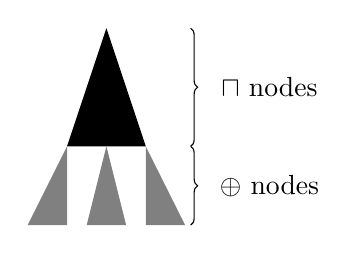
\begin{tikzpicture}[scale=0.5]
            \path[fill,black] (0,0) -- (1, -3) -- (-1, -3) -- (0,0) ;
            \path[fill,gray ] (1, -3) -- (2, -5) -- (1, -5) ;
            \path[fill,gray ] (-1, -3) -- (-2, -5) -- (-1, -5) ;
            \path[fill,gray ] (0, -3) -- (-0.5, -5) -- (0.5, -5) ;

            \draw [decorate,decoration={brace},xshift=4pt,yshift=0pt]
                (2,0) -- (2,-3) node [black,midway,xshift=1cm] 
                {$\sqcap$ nodes};
            \draw [decorate,decoration={brace},xshift=4pt,yshift=0pt]
                (2,-3) -- (2,-5) node [black,midway,xshift=1cm] 
                {$\oplus$ nodes};
        \end{tikzpicture} 
    \end{center}

    Because we now that $\sqeq_b$ satisfies $\mathcal{T}$, we can 
    always transform an inequality $t \sqeq_b t'$ into an inequality 
    where both trees are of the previously defined shape: with a finite 
    heap of $\sqcap$-nodes and possibly infinite subtrees of $\oplus$-nodes.

    Assume that we are given two trees $t$ and $t'$ with a finite number 
    of $\sqcap$-nodes such that $t \sqeq_b t'$. It suffices to show that 
    the equivalent trees with a finite heap of $\sqcap$-nodes and subtrees 
    of $\oplus$-nodes are related for $\sqeq_\mathcal{T}$. But because 
    of the laws of the demonic-choice operator, it is enough to prove that 
    for all $\oplus$-nodes subtree of $t'$, there exists a $\oplus$-nodes
    subtree of $t$ that is under it for $\sqeq_\mathcal{T}$. This is illustrated 
    in the following figure, where arrows symbolises an inequality relation for
    $\sqeq_\mathcal{T}$:

    \begin{center}
        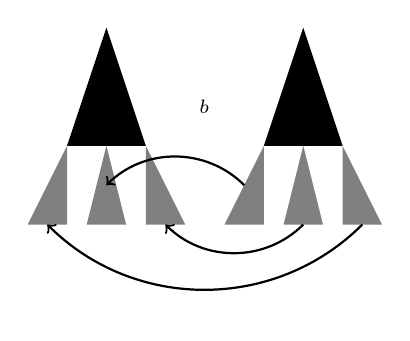
\begin{tikzpicture}[scale=0.5]
            \path[fill,black] (0,0) -- (1, -3) -- (-1, -3) -- (0,0) ;
            \path[fill,gray ] (1, -3) -- (2, -5) -- (1, -5) ;
            \path[fill,gray ] (-1, -3) -- (-2, -5) -- (-1, -5) ;
            \path[fill,gray ] (0, -3) -- (-0.5, -5) -- (0.5, -5) ;

            \draw (2.5,-2) node {$\sqeq_b$};

            \path[fill,black] (5,0) -- (6, -3) -- (4, -3) -- (5,0) ;
            \path[fill,gray ] (6, -3) -- (7, -5) -- (6, -5) ;
            \path[fill,gray ] (4, -3) -- (3, -5) -- (4, -5) ;
            \path[fill,gray ] (5, -3) -- (4.5, -5) -- (5.5, -5) ;


            \path[thick,->] (5,-5) edge [bend left=45] (1.5,-5) ;
            \path[thick,->] (6.5,-5) edge [bend left=45] (-1.5,-5) ;
            \path[thick,->] (3.5,-4) edge [bend right=45] (0,-4) ;
        \end{tikzpicture} 
    \end{center}
    
    However, it is not always possible to find a matching $\oplus$-subtree 
    in $t$ for all $\oplus$-subtrees in $t'$. The key to overcome this 
    issue is to notice  that $a \sqcap (a \oplus b)
    \sqcap b$ is provably equivalent to $a \sqcap b$ in the theory
    $\mathcal{T}$ \cite{mislove2004axioms}. 
    An $\oplus$-combination of a set of trees $t_1, \dots, t_n$
    is determined by a tree (possibly infinite) 
    with only $\oplus$-nodes and leaves numbered from $1$ to $n$,
    and the combination itself is obtained by substituting the leaf $i$
    in this tree by the tree $t_i$.
    The previous result with only two trees can be extended to prove that any
    $\oplus$-combination
    of $\oplus$-subtrees of $t$ can be added as a new
    $\oplus$-subtree while being provably equivalent in $\mathcal{T}$.



    Thus, it is enough to find for all $\oplus$-subtrees in $t'$ an 
    $\oplus$-combination of $\oplus$-subtrees in $t$ that is 
    under it for $\sqeq_\mathcal{T}$ as illustrated in the following 
    Figure:

    \begin{center}
        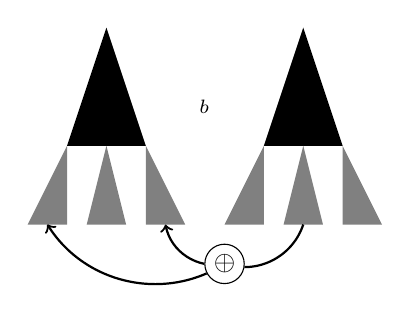
\begin{tikzpicture}[scale=0.5]
            \path[fill,black] (0,0) -- (1, -3) -- (-1, -3) -- (0,0) ;
            \path[fill,gray ] (1, -3) -- (2, -5) -- (1, -5) ;
            \path[fill,gray ] (-1, -3) -- (-2, -5) -- (-1, -5) ;
            \path[fill,gray ] (0, -3) -- (-0.5, -5) -- (0.5, -5) ;

            \draw (2.5,-2) node {$\sqeq_b$};

            \path[fill,black] (5,0) -- (6, -3) -- (4, -3) -- (5,0) ;
            \path[fill,gray ] (6, -3) -- (7, -5) -- (6, -5) ;
            \path[fill,gray ] (4, -3) -- (3, -5) -- (4, -5) ;
            \path[fill,gray ] (5, -3) -- (4.5, -5) -- (5.5, -5) ;


            \path[thick] (5,-5) edge [bend left=45] (3,-6) ;
            \path[thick,->] (3,-6) edge [bend left=45] (1.5,-5) ;
            \path[thick,->] (3,-6) edge [bend left=45] (-1.5,-5) ;
            \draw[fill,white] (3,-6) circle (0.5) ;
            \draw (3,-6) circle (0.5) ;
            \draw (3,-6) node {$\oplus$};
        \end{tikzpicture} 
    \end{center}

    In order to continue the proof, we use the fact that the operational 
    preorder on trees containing only $\oplus$-nodes can be captured 
    by translating the tree into a linear function from $(\mathbb{N}_\bot \to
    \overline{\mathbb{R}_+})$ to $\overline{\mathbb{R}_+}$ because 
    there is no $\sqcap$-node and therefore changing strategy does not 
    change the outcome, which allows us to remove the infimum. Using this 
    correspondence, we are going to prove two separate results:

    \begin{enumerate}[(i)]
        \item If $t \sqeq_b t'$ both with a finite number of $\sqcap$-nodes,
            then the $\oplus$-subtrees extracted from them 
            can be translated into linear functions from $(\mathbb{N}_\bot \to
            \overline{\mathbb{R}_+}) \to \overline{\mathbb{R}_+}$. 
            For all $\oplus$-subtree 
            of $t'$, the corresponding linear function is above 
            a \emph{convex combination} of linear functions corresponding 
            to $\oplus$-subtrees of $t$.

        \item A linear combination of functions corresponding to 
            $\oplus$-subtrees can be obtained as the linear 
            function corresponding to an $\oplus$-combination 
            of the said subtrees.

        \item If a probabilistic tree $t$ is under a probabilistic tree $t'$ 
            for $\sqeq_b$ then it is provable that they are also related for
            $\sqeq_\mathcal{T}$.
    \end{enumerate}

    It is clear that if both steps are proven, given an $\oplus$-subtree of $t'$
    it suffices to use (i) 
    to find a convex combination of linear functions that is under its
    corresponding linear function, and then use (ii) to convert this 
    back into trees combined with $\oplus$, allowing us to conclude using 
    the last point (iii).

    The last point (iii) is referring to the completeness result already proven 
    using only the probabilistic choice in Lemma \ref{lem:probpreo}, because 
    the theory $\mathcal{T}$ is an extension of the theory containing only 
    probabilistic choice, the proofs transported.

    Proving the point (ii) is simply proving that any distribution of probability 
    over a finite subset $U$ of $\mathbb{N}$
    can be obtained using an infinite binary tree of $\oplus$-nodes and 
    leaves in $U \cup \{ \bot \}$.

    The proof of point (i) is more complex, and requires several technical 
    tools \cite{JGL-mscs16}. We fix an arbitrary $\oplus$-subtree of $t'$ and
    write $L$ for the associated linear function, we also write 
    $L_1, \dots, L_n$ the linear functions associated to $\oplus$-subtrees of
    $t$. By definition of the operational preorder $\sqeq_b$ and because 
    of the shape of the tree we know that:

    \begin{equation*}
        \forall h : \mathbb{N} \to \overline{\mathbb{R}_+}, 
            \min (L_1 (h), \dots, L_n (h)) \leq L(h)
    \end{equation*}

    We want to prove that this implies that there exists a convex combination 
    of $L_1, \dots, L_n$ that is under $L$ for any $h$. We write 
    $A = \operatorname{Conv}\left( \{ M \text{ linear } ~|~ \exists i, M \geq
    L_i \} \right)$, and our goal is equivalent to proving that $L \in A$. Assuming it 
    is not the case, we will find a contraction when looking at the 
    set of linear functions under $L$: $B = \{ M \text{ linear } ~|~ M \leq L
    \}$.

    Indeed, because $L \not \in A$, it is easy to show that $B \cap A =
    \emptyset$. However, referring to \cite{JGL-mscs16} and \cite{KeimelP2016} 
    both are \emph{convex} and \emph{closed} set of a locally-convex topological 
    cone: the cone of linear functions from $(\mathbb{N}_\bot \to
    \overline{\mathbb{R}_+})$ to $\overline{\mathbb{R}_+}$. It is therefore 
    possible to use a convex separation theorem \cite{JGL-mscs16} and build 
    a linear functional $\Lambda$ from the cone of linear functions to
    $\overline{\mathbb{R}_+}$ such that there exists a real number $r$
    and:
    \begin{align*}
        \forall M \in B, \Lambda (M) < 1 < r \\
        \forall M \in A, \Lambda (M) > r > 1
    \end{align*}

    Now using the Schröder-Simpson representation theorem \cite{SchroderS06}, 
    there exists a test function $h$ such that for all linear functions $M$
    in our cone:
    \begin{equation*}
        \Lambda (M) = M(h)
    \end{equation*}

    But we can therefore deduce that for all $i$, $\Lambda (L_i) > r > 1 > \Lambda (L)$
    meaning that $L_i (h) > L(h)$ for all $i$. This is a contradiction with 
    the inequality derived from the operational preorder, and therefore $L \in
    A$, allowing us to conclude.

    \vspace{2em}

    It is now proven that if $t$ and $t'$ have a finite number of $\sqcap$-nodes 
    then $t \sqeq_b t'$ implies $t \sqeq_\mathcal{T} t'$. To extend this result 
    to trees with an infinite number of $\sqcap$-nodes, we are going to use 
    the admissibility rule of $\sqeq_\mathcal{T}$. Assume $t$ and $t'$ are 
    two trees such that $t \sqeq_b t'$, we can build two ascending chains 
    of \emph{finite} trees $(t_i)$ and $(t_i')$ having as least upper bounds 
    respectively $t$ and $t'$. The goal is to prove that $t \sqeq_\mathcal{T}
    t'$, however, it is not possible to directly prove that $t_i
    \sqeq_\mathcal{T} t_i'$ and conclude using admissibility.
    
    We are instead going to use several approximation steps to obtain
    the desired result. First of all, we are going to define 
    $a^n$ where $a$ is a tree and $n$ a natural number as follows:

    \begin{equation*}
        \begin{cases}
            a^0 &= \bot \\
            a^{n+1} &= a \oplus a^{n}
        \end{cases}
    \end{equation*}

    This operator is useful to obtain \emph{strict} inequalities at any test function $h$, 
    indeed it is easy to see that:

    \begin{equation*}
        \inf_{s \in \mathcal{S}} F(a^n,s,h) = 
        \inf_{s \in \mathcal{S}} \frac{2^n - 1}{2} F(a,s,h) 
        < 
        \inf_{s \in \mathcal{S}} F(a,s,h)
    \end{equation*}

    Moreover we showed that the function
    $\llbracket \cdot \rrbracket : t \mapsto \inf_{s \in S} F (t,s,h)$
    is Scott-continuous in $t$ in Lemma \ref{lem:mixedscottcontinuous}.
    
    It is now possible to look at the ascending chains, and 
    notice that:

    \begin{align*}
        \llbracket t_i \oplus (t_i')^n \rrbracket(h) &= \frac{\llbracket t_i
        \rrbracket(h) + \llbracket (t_i')^n \rrbracket (h)}{2} \\
        &< 
        \frac{\llbracket t_i \rrbracket(h) + \llbracket t_i' \rrbracket (h)}{2} \\
        &\leq \llbracket t' \rrbracket(h)
    \end{align*}
    
    Using the Scott-continuity of $\llbracket \cdot \rrbracket$ allows us to 
    rewrite it in the following way:

    \begin{equation*}
        \llbracket t_i \oplus (t_i')^n \rrbracket < \sup_i \llbracket t_i' \rrbracket
    \end{equation*}

    Therefore for all $i$ there exists a $j>i$ such that:

    \begin{equation*}
        \llbracket t_i \oplus (t_i')^n \rrbracket < \llbracket t_j' \rrbracket
    \end{equation*}

    Because all trees in this equation are finite, and the inequality is
    equivalent to being related for $\sqeq_b$, we can use the previous 
    result on trees with finite number of $\sqcap$-nodes to conclude:

    \begin{equation*}
        t_i \oplus (t_i')^n \sqeq_\mathcal{T} t_j'
    \end{equation*}

    Now using the admissibility property while fixing $n$, we can deduce that:

    \begin{equation*}
        t \oplus (t')^n \sqeq_\mathcal{T} t'
    \end{equation*}

    Using again the admissibility property, this time on the sequence $(t')^n$ 
    we can obtain:

    \begin{equation*}
        t \oplus (t') \sqeq_\mathcal{T} t'
    \end{equation*}

    Now using the least-fixed-point rule from the probability theory we can 
    conclude:

    \begin{equation*}
        t \sqeq_\mathcal{T} t'
    \end{equation*}
    \qed
\end{proof}

\subsection{Counterexample for the simpler preorder}

From a domain perspective, it was natural to consider 
the functional domain using arbitrary test functions 
$h$ from $\mathbb{N}_\bot$ to $\overline{\mathbb{R}_+}$
because they arise from a bidual construction \cite{JGL-mscs16}. 
From a Markov Decision Process point of view 
however, we can ask ourselves if restricting 
to \emph{characteristic functions} is enough. 
Indeed, this leads us with a better understanding 
of the process, where the objective is simply
to \emph{avoid} one set with the highest probability 
possible. The preorder would then become:

\begin{equation*}
    t \sqeq_b t' \iff \forall U \subseteq \mathbb{N}, 
    \inf_{ s \in \mathcal{S}} F (t,s, \chi_U ) \leq \inf_{s \in \mathcal{S}}
    F (t',s, \chi_U )
\end{equation*}

This idea, while appealing is not possible because 
the following inequation cannot be true in general
(see \cite{Mislove2000} and \cite{mislove2004axioms}) without 
implying that probabilistic choice behaves like demonic choice: 

\begin{equation*}
    (a +_p b) \sqcup c \neq 
    (a \sqcup c) +_p (b \sqcup c)
\end{equation*}

However, for our preorder using only sets, the 
two trees in Figure \ref{fig:counterexampletree} that 
are obtained by replacing $a,b,c$ 
by $1,2,3$ are behaving in the same way for any 
characteristic function: the lowest probability to 
be inside a given subset of $\{1,2,3\}$ is the same 
for both trees.

\begin{figure}[h]

    \begin{center}
        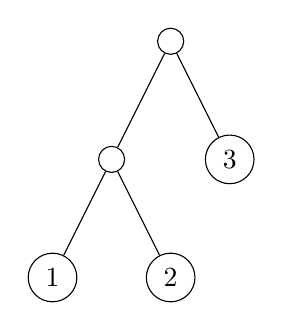
\begin{tikzpicture}
            \node [circle,draw] (z){$\orEff$}
                child { 
                    node [circle,draw] (a) {$\prEff$}
                    child { node[circle,draw] (b) {$1$} } 
                    child { node[circle,draw] (c) {$2$} }
                }
                child {
                    node [circle,draw] (d) {$3$}    
                };
        \end{tikzpicture}
        \hspace{2em}
        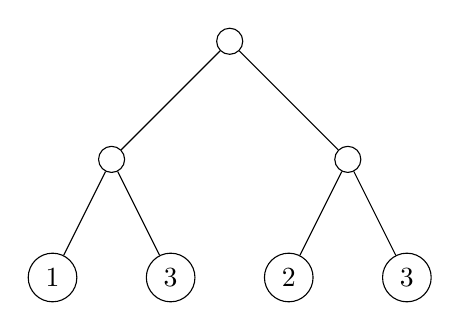
\begin{tikzpicture}[level 1/.style={sibling distance=3cm},
                            level 2/.style={sibling distance=1.5cm}]
            \node [circle,draw] (z){$\prEff$}
                child { 
                    node [circle,draw] (h) {$\orEff$}
                    child { node[circle,draw] (b) {$1$} } 
                    child { node[circle,draw] (c) {$3$} }
                }
                child {
                    node [circle,draw] (g) {$\orEff$}
                    child { node[circle,draw] (e) {$2$} } 
                    child { node[circle,draw] (f) {$3$} }
                };
        \end{tikzpicture}
    \end{center}

    \begin{equation*}
        \orEff (\prEff (1,2), 3) \quad \quad \prEff (\orEff (1,3), \orEff (2,3))
    \end{equation*}
    \caption{The two trees from the counterexample}
    \label{fig:counterexampletree}
\end{figure}

We can see that the two trees in Figure \ref{fig:counterexampletree} 
have the same interpretation in terms of characteristic functions,
and the result from \cite{Mislove2000} shows us that a reasonable 
preorder shouldn't equate them. But we have an explicit 
cost function $h$ that shows that the interpretation in terms of 
expectancies is different for the two trees:

\begin{equation*}
    h (i) = \begin{cases}
        1 & \text{ when } i = 1 \\
        8 & \text{ when } i = 2 \\
        2 & \text{ when } i = 3 \\
        0 & \text{ otherwise } 
    \end{cases}
\end{equation*}

This function can distinguish between the two trees 
because the least expected cost for the first one is $1/4$
where the least expected cost for the second one is $3/16$.

The choice of costs for $h$ is not random: we can divide 
everything by $8$ to get costs of the form $1/2^i$ 
and build an actual substitution $\sigma$ where $\sigma(i)$ 
is the tree where the probability to get $1$ is $h(i)/8$.
